\documentclass[msthesis.tex]{subfiles}

\begin{document}
\chapter{Background}
Non-invasive neuroimaging techniques have become indispensable tools to understand cognitive processes and neurological disease pathology. \Gls{dMRI} is a new type of imaging modality often used to produce highly detailed anatomical images. It is suitable for looking at soft tissues such as those in the nervous system. White matter tractography from \gls{dMRI} scans enables the inference of structural connectivity patterns between brain regions. Analysis of individual differences in structural brain connectivity is relevant to understand emotion, behavior, and cognition. 

Individual differences in neuroimaging are often evaluated using machine learning classifiers. Classification based on neuroimaging techniques is an intricate task. It suffers from the \textit{curse of dimensionality} and lack of interpretability. Using graph based techniques along with feature selection methods can help establish neurobiological correspondence of the decision made by a classifier. 

This chapter describes the prerequisites required to understand the implementation in \autoref{chap:methods}. In the first few sections, the technical details of imaging using \gls{MRI} and \gls{dMRI} will be presented. Subsequent sections give an introduction to the prior work relevant for classification based on structural brain connectivity.

\section{Magnetic Resonance Imaging}
\gls{MRI} is a non-invasive imaging technology that can produce 3-dimensional detailed anatomical images \citep{mcrobbie_moore_graves_prince_2006}. This technique is based on the \gls{NMR} principle. \Gls{NMR} a physical phenomenon in which nuclei respond to a combination of a constant and a weakly oscillating magnetic field by producing a signal at their resonant frequency. The difference between the magnetic properties of different tissue types subjected to an external magnetic field is used to generate images of biological specimens. Such electromagnetic properties are used to form images since the human body is 65\% water ($H_2O$). Water has an innate dipole moment of $1.84 D$ and its hydrogen nuclei act like little magnets since they have an odd number of protons and non-zero net spin. 

In normal conditions (\cref{mriphysics}.a), i.e. in the absence of an external magnetic field the spins of the hydrogen nuclei are randomly oriented and appear to cancel out each other when observed as an ensemble. Once the external field is applied, the hydrogen nuclei exhibit their paramagnetic nature and gain a net magnetization in the direction of the external magnetic field. This magnetization is called as the longitudinal magnetization. The initial longitudinal magnetization can be represented using the following equation:
\begin{equation}
       \Vec{M_o} = \mu \Vec{B_0}
\end{equation}
where $M_0$ is the net magnetization, $\mu$ is the magnetic permeability or the inertia of a material to get magnetized and $B_0$ is the external magnetic field. According to \cref{mriphysics}.a it can be seen that the direction of $B_0$ defines the coordinate system for the imaging experiment. The transverse plane is defined as the plane perpendicular to the direction of $B_0$. The magnetization in this plane is termed as the transverse magnetization. In the presence of the external static magnetic field, the individual nuclei are precessing (rotating around their axis) with a frequency known as the Larmour frequency, which can be expressed by the equation:
\begin{equation}
    \omega_0 = \gamma B_0
    \label{larmour}
\end{equation}
where $\omega_o$ represents the frequency, $\gamma$ represents the gyromagnetic ration and $B_0$ the external field.
\begin{figure}
\centering
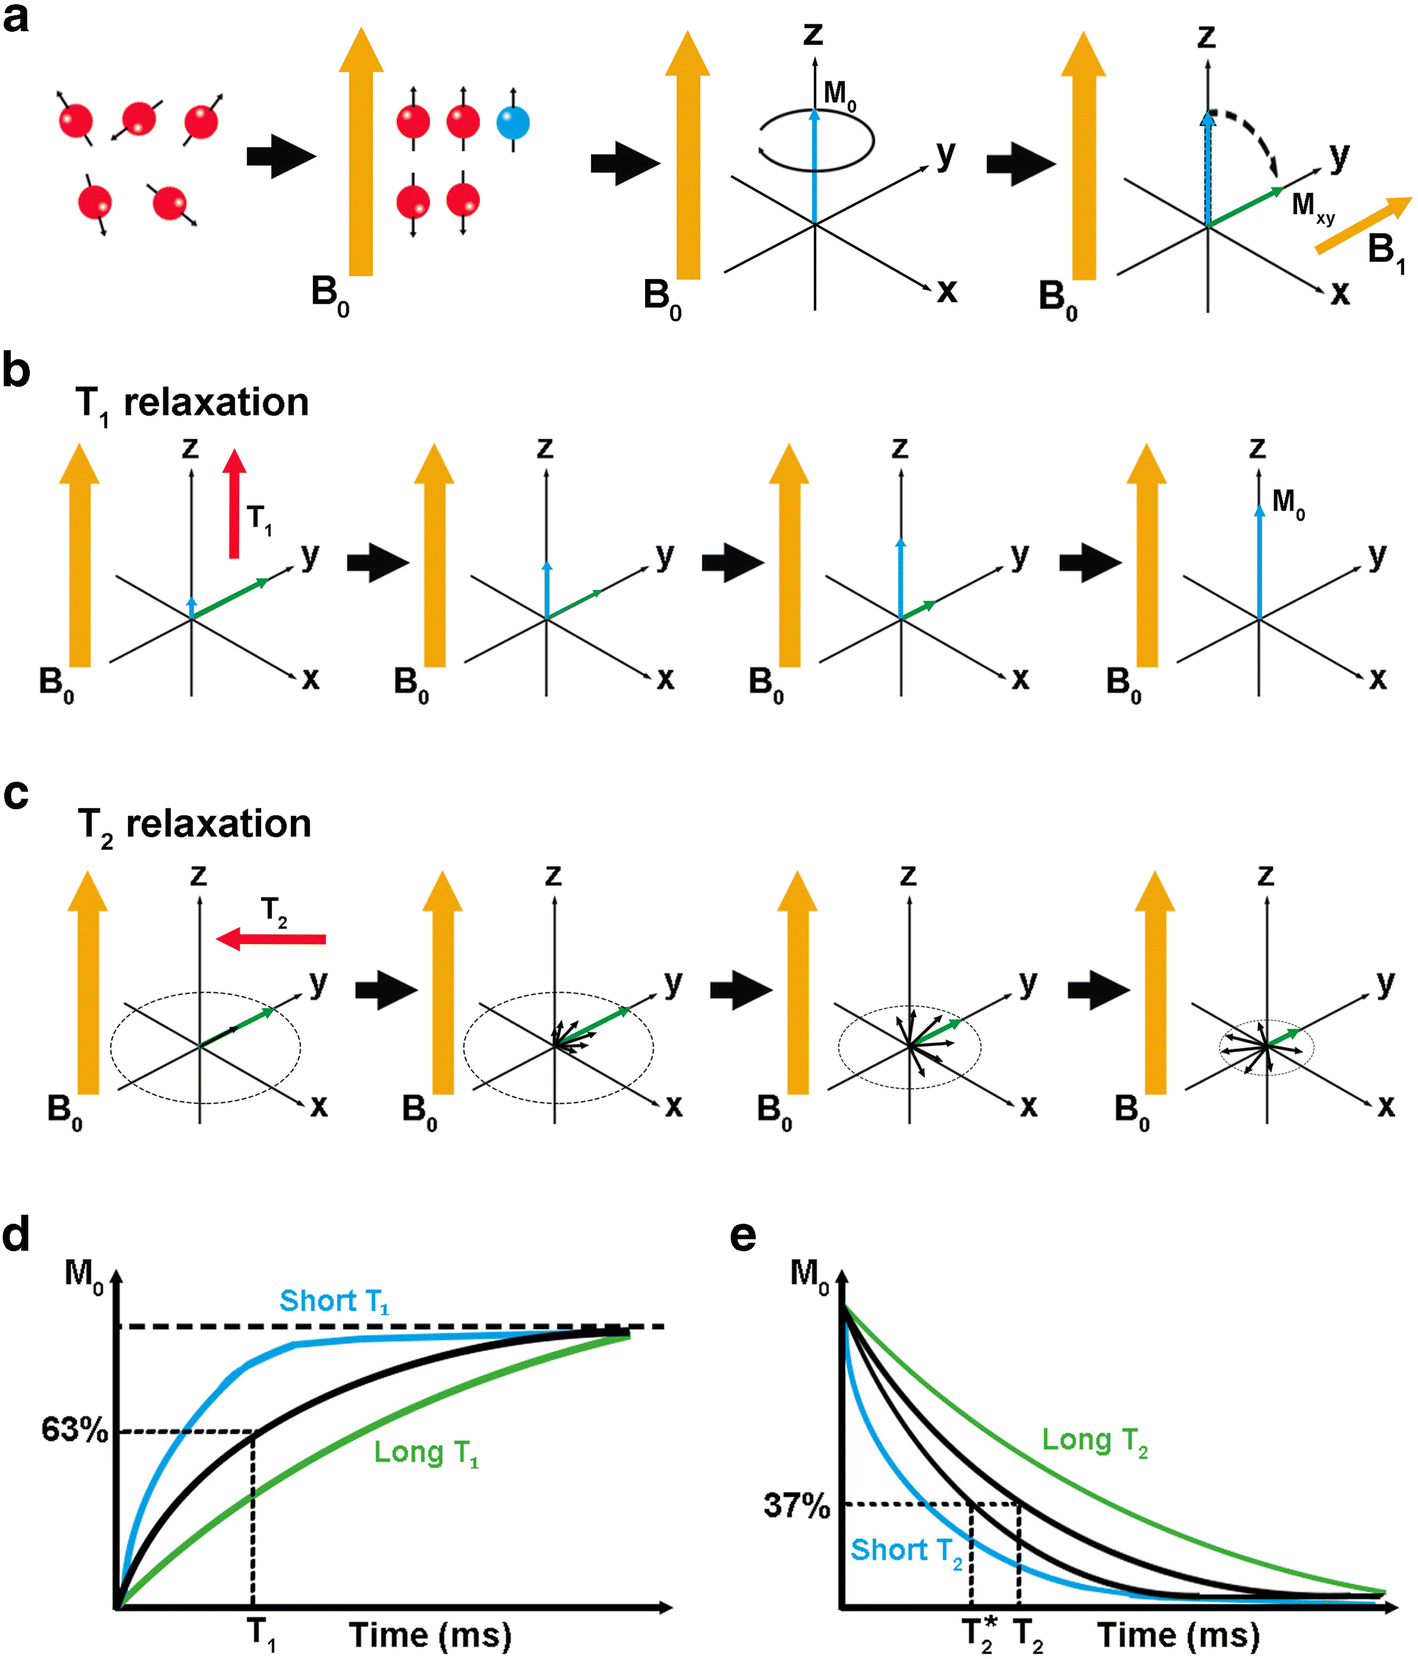
\includegraphics[width=0.847\textwidth]{images/mri1.png}
\caption{Figure from \cite{Mastrogiacomo2019}. (a) At first the magnetic moments of the individual nuclei are oriented randomly and cancel out each other. In the presence of an external field $B_0$ they gain a net magnetization. With the presence of the external RF pulse the phase of the net magnetization is changed and magnetic resonance is said to occur. (b) Describes process of T1 relaxation in which the net magnetization starts to align along the static magnetic field $B_0$. (c) Describes T2 relaxation or the dephasing of magnetization in the transverse plane. (d) Illustrates that the value of the T1 constant is the time required to achieve 63\% of the longitudinal magnetization. (e) The time constant T2 is the time required for the magnetization to fall to 1/e of its value. In (d) and (e) the blue lines represent tissues containing fat while the green lines represent fluids such as \gls{CSF}.}
\label{mriphysics}
\end{figure}

An oscillating field operating at the Larmour frequency \cref{larmour}) is then added to the static magnetic field using an \gls{RF1} coil. This field is termed as $B_1$ in \cref{mriphysics}.a. The $B_1$ field causes the direction of the net magnetization vector to get altered i.e. ‘flipped’ or ‘tipped’ out of alignment with $B_0$. The net magnetization gets tipped towards $B_1$ with the angle of rotation termed as the flip angle. The RF pulse exerts a torque which can be mathematically expressed as:
\begin{equation}
    \Vec{\tau} = \Vec{m} \times \Vec{B_1}
\end{equation}
where $\Vec{m}$ is the magnetic moment and the $ \Vec{B_1}$ is the applied magnetic field. The flipping does not bring all the spins in phase with each other but causes the net magnetization to flip onto the transverse plane ($M_{xy}$ in \cref{mriphysics}.a). The magnetization $M_{xy}$ then precesses in this plane. It is important to note that the net magnetization does not precess until an external force disturbs its equilibrium position of alignment with the static magnetic field. When the magnetization precesses, magnetic resonance is said to occur.

After this, the \gls{RF1} pulse is switched off which causes the tissue molecules to return to their original state and is termed as the relaxation phase. The relaxation is due to the release of electromagnetic energy into the environment to attain thermal equilibrium. This release of electromagnetic energy is what forms the signal for the receiver coil. \cite{PhysRev.70.460} introduced two time constants to measure the relaxation phase, T1 and T2.

The constant T1 measures the growth of the longitudinal component ($M_z$, \cref{mriphysics}.b) with T1 relaxation being termed as the process by which the net magnetization aligns itself along the direction of the original magnetic field. The T2 constant measures the decay of the transverse component of the magnetization (\cref{mriphysics}.c). The value of T2 reflects the time required for the magnetization to fall to $\frac{1}{e}$ or 37\% of its original value, illustrated in \cref{mriphysics}.e. Since there can be inhomogeneities inside the \gls{MRI} scanner, another constant $T2^*$ is measured as the T2 time observed while taking the recording to account for such effects. During the resonance phenomena, the magnetization has components in different directions which can be expressed in terms of the time constants and time lapse ($t$) of the experiment.
\begin{equation}
    M_x(t) = M_o e^{\frac{−t}{T2}} \sin{ \omega t}
    \label{mx}
\end{equation}
\begin{equation}
    M_y(t) = M_o e^{\frac{-t}{T2}} \cos{\omega {t}}
    \label{my}
\end{equation}
\begin{equation}
    M_z(t) = M_o (1 − e^{{\frac{−t}{T1}}})
    \label{mz}
\end{equation}
Where $M_x$ ,$M_y$, $M_z$ are the magnetizations along the x,y and z directions and $M_0$ is the magnetization induced by the applied static magnetic field $B_0$. From \cref{mz} it is clear that the T1 constant measure the time required to gain the original magnetization, i.e. $t=T1 \implies M_z = M_0$ and $t=T2 \implies M_{xy} = \frac{M_0}{\cos{\omega T2}}$. The differences in T1 and T2 times of different tissues (\cref{mriphysics}.d and \cref{mriphysics}.e) are often used to generate a contrast for image formation.

Image contrasts are indirectly controlled using \gls{TR} and \gls{TE} in a sequence. \Gls{TR} is defined as the time taken between successive excitations of the same region. \Gls{TE} measures time between excitation and signal measurement. Short \gls{TR} and short \gls{TE} generate T1 weighted images while long \gls{TR} and long \gls{TE} generate T2 weighted images.

Different types of brain tissues have different T1 and T2 values. Short T1 times are seen in fat molecules because of their complex structure. The intricacies of saturated molecules lead to flexions and roations which might occur at the Larmour frequency. This makes it easier for the magnetization to return to the initial state (longitudinal orientation). Longer T1 times are observed in comparatively freely diffusing mediums such as \gls{CSF}. Such fluids appear dark on T1-weighted images due to longer T1 times while fat molecules appear bright with the same diffusion weighting. Fat molecules appear lighter on T2-weighted images due to short T2 time while the \gls{CSF} appears bright since it has long T2 times.

\subsection{Image formation}

An \gls{MRI} scan needs to represent the 3D nature of specimen under study. Inside an \gls{MRI} scanner, the gradient coils are used to alter the magnetic field along the different spatial directions. This ensures that different slices of the biological structure to resonate at different frequencies. The signal from all the slices is then detected by receiver coils that recognize only the transverse magnetization. In neuroimaging studies this signal needs spatial encoding to transmit information about the millions of voxels at different spatial locations in the brain.

\begin{figure}
    \centering
    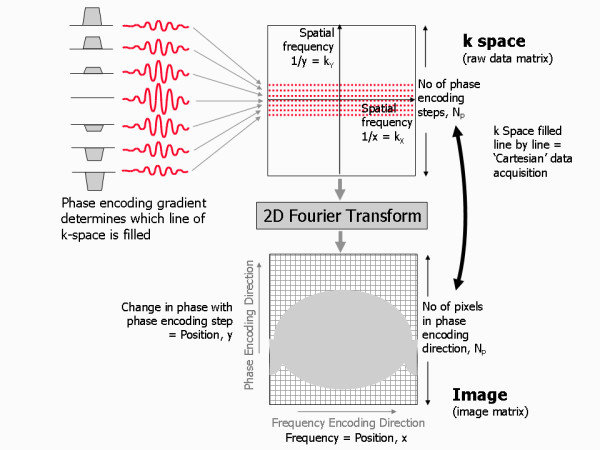
\includegraphics[width=\textwidth]{images/img_reconstruction.jpg}
    \caption{Image from \cite{MRIrecon} summarising the reconstruction of an encoded \gls{MRI} signal in 2D. A  2D slice has been selected using the gradient $G_z$. The phase is encoded along the y direction and the frequency is encoded along the x direction. Each phase encoding step is used to populate the k-space. The number of such steps determines the number of pixels along the y direction in the reconstructed image. The relationship between the k-space points and the points in reconstructed image space is such that $k_x =1/x$ and $k_y= 1/y$. In the k-space, each line parallel to the $k_x$ axis corresponds to a separate MRI signal. The number of such signals is the number of times the pulse sequence is repeated. The location on the x-axis determines the time during signal acquisition. Each line parallel to the $k_y$ axis corresponds to the amplitude and duration of the phase encoding direction (gradient) at each phase encoding step (y coordinate).}
    \label{fig:mri_img}
\end{figure}

It is known that in order to form the 3D image the magnetic gradients are applied in the x,y,z directions. This formalism results in each voxel possessing a different Larmour frequency and the phenomenon can be termed as spatial encoding. 
\begin{equation}
        \label{eq:larmour_grad}
          \omega = \gamma(B_0 + G(x, y, z))
     \end{equation}
       
According to \cref{eq:larmour_grad}, it is evident that there is a direct relation between the gradient field and the Larmour frequency. Usually the gradient for the slice selection is applied along the z-direction. For better understanding a simpler case of 2D image reconstruction has been explained in the \cref{fig:mri_img} where the phase encoding gradients are applied in a direction perpendicular to the frequency encoding gradients.

The \gls{RF1} coils in the \gls{MRI} scanner detects a signal containing a mixture of frequencies specific for each slice and each phase encoding step. The distribution of frequencies is determined using a Fourier transform. This distribution is then used to fill what is called as the k-space. The 2D k-space in \cref{fig:mri_img} is used to elucidate the components of the frequency. The intensity of a point in the space represents the contribution of the frequency $(k_x,k_y)$ in the signal. For each combination of $(k_x, k_y)$ in the k-space the scanner camera takes only one picture (one filter per voxel). It then estimates the actual intensities at different locations using an inverse Fourier transform. There is a one-to-one correspondence of the pixel in the k-space to the image space. Every pixel in the 2D k-space image maps to only one pixel in the reconstructed 2D image. However, it is not necessary that the locations in both the images are exactly the same. This mapping using a Fourier transform is then extrapolated in 3D in order to obtain the image of the whole organ such as the brain. Any weighting such as T1w or T2w can be given in order to generate the image after the transformation has taken place.

Another important concept for image formation is that of \gls{FOV}. It refers to the distance over which an \gls{MRI} signal is acquired or displayed. The defined \gls{FOV} determines the pixel width (determined by the phase encoding y direction in \cref{fig:mri_img}) given by $\Delta k = 1/FOV$. 

\subsection{Diffusion MRI}

\gls{dMRI} is an \textit{in-vivo}, non-invasive imaging modality that used to create high-resolution structural images of biological tissues. It measures the non-homogeneity of water diffusion in tissues to probe their microstructure \citep{ghosh2015survey}. One of the most important applications of \gls{dMRI} is to map the white-matter fiber tracts in the brain. As compared to other \gls{MRI} techniques such as \gls{fMRI} it does not suffer from an issue of low resolution and low \gls{SNR} \citep{wong2016}. 

``Diffusion'' is defined as the net movement of a substance from a region of higher concentration to a region of lower concentration. In a homogeneous medium, the diffusion of water molecules is isotropic, i.e. the molecules can move in any direction with equal probability. They exhibit random walk behavior which is explained by Brownian motion \citep{Brogioli_2000}.

The environment inside a biological tissue is complex and the diffusion of water molecules becomes anisotropic due to the hindrances imposed by cellular membranes. This causes water molecules in the extracellular environment to experience relatively free diffusion and the ones in the intra-cellular environment experience restricted diffusion \citep{toennies2017guide}. This diffusion anisotropy is encoded into the MRI signal using spatial and temporal variation (gradients) in the magnetic field. This means that the alignment of the molecules is influenced by the diffusion direction. The \gls{MRI} signal is said to be ``Diffusion Weighted'' due to signal attenuation introduced by the magnetic field gradients. 


\subsubsection{Diffusion Weighted Imaging}
\begin{figure}
    \centering
    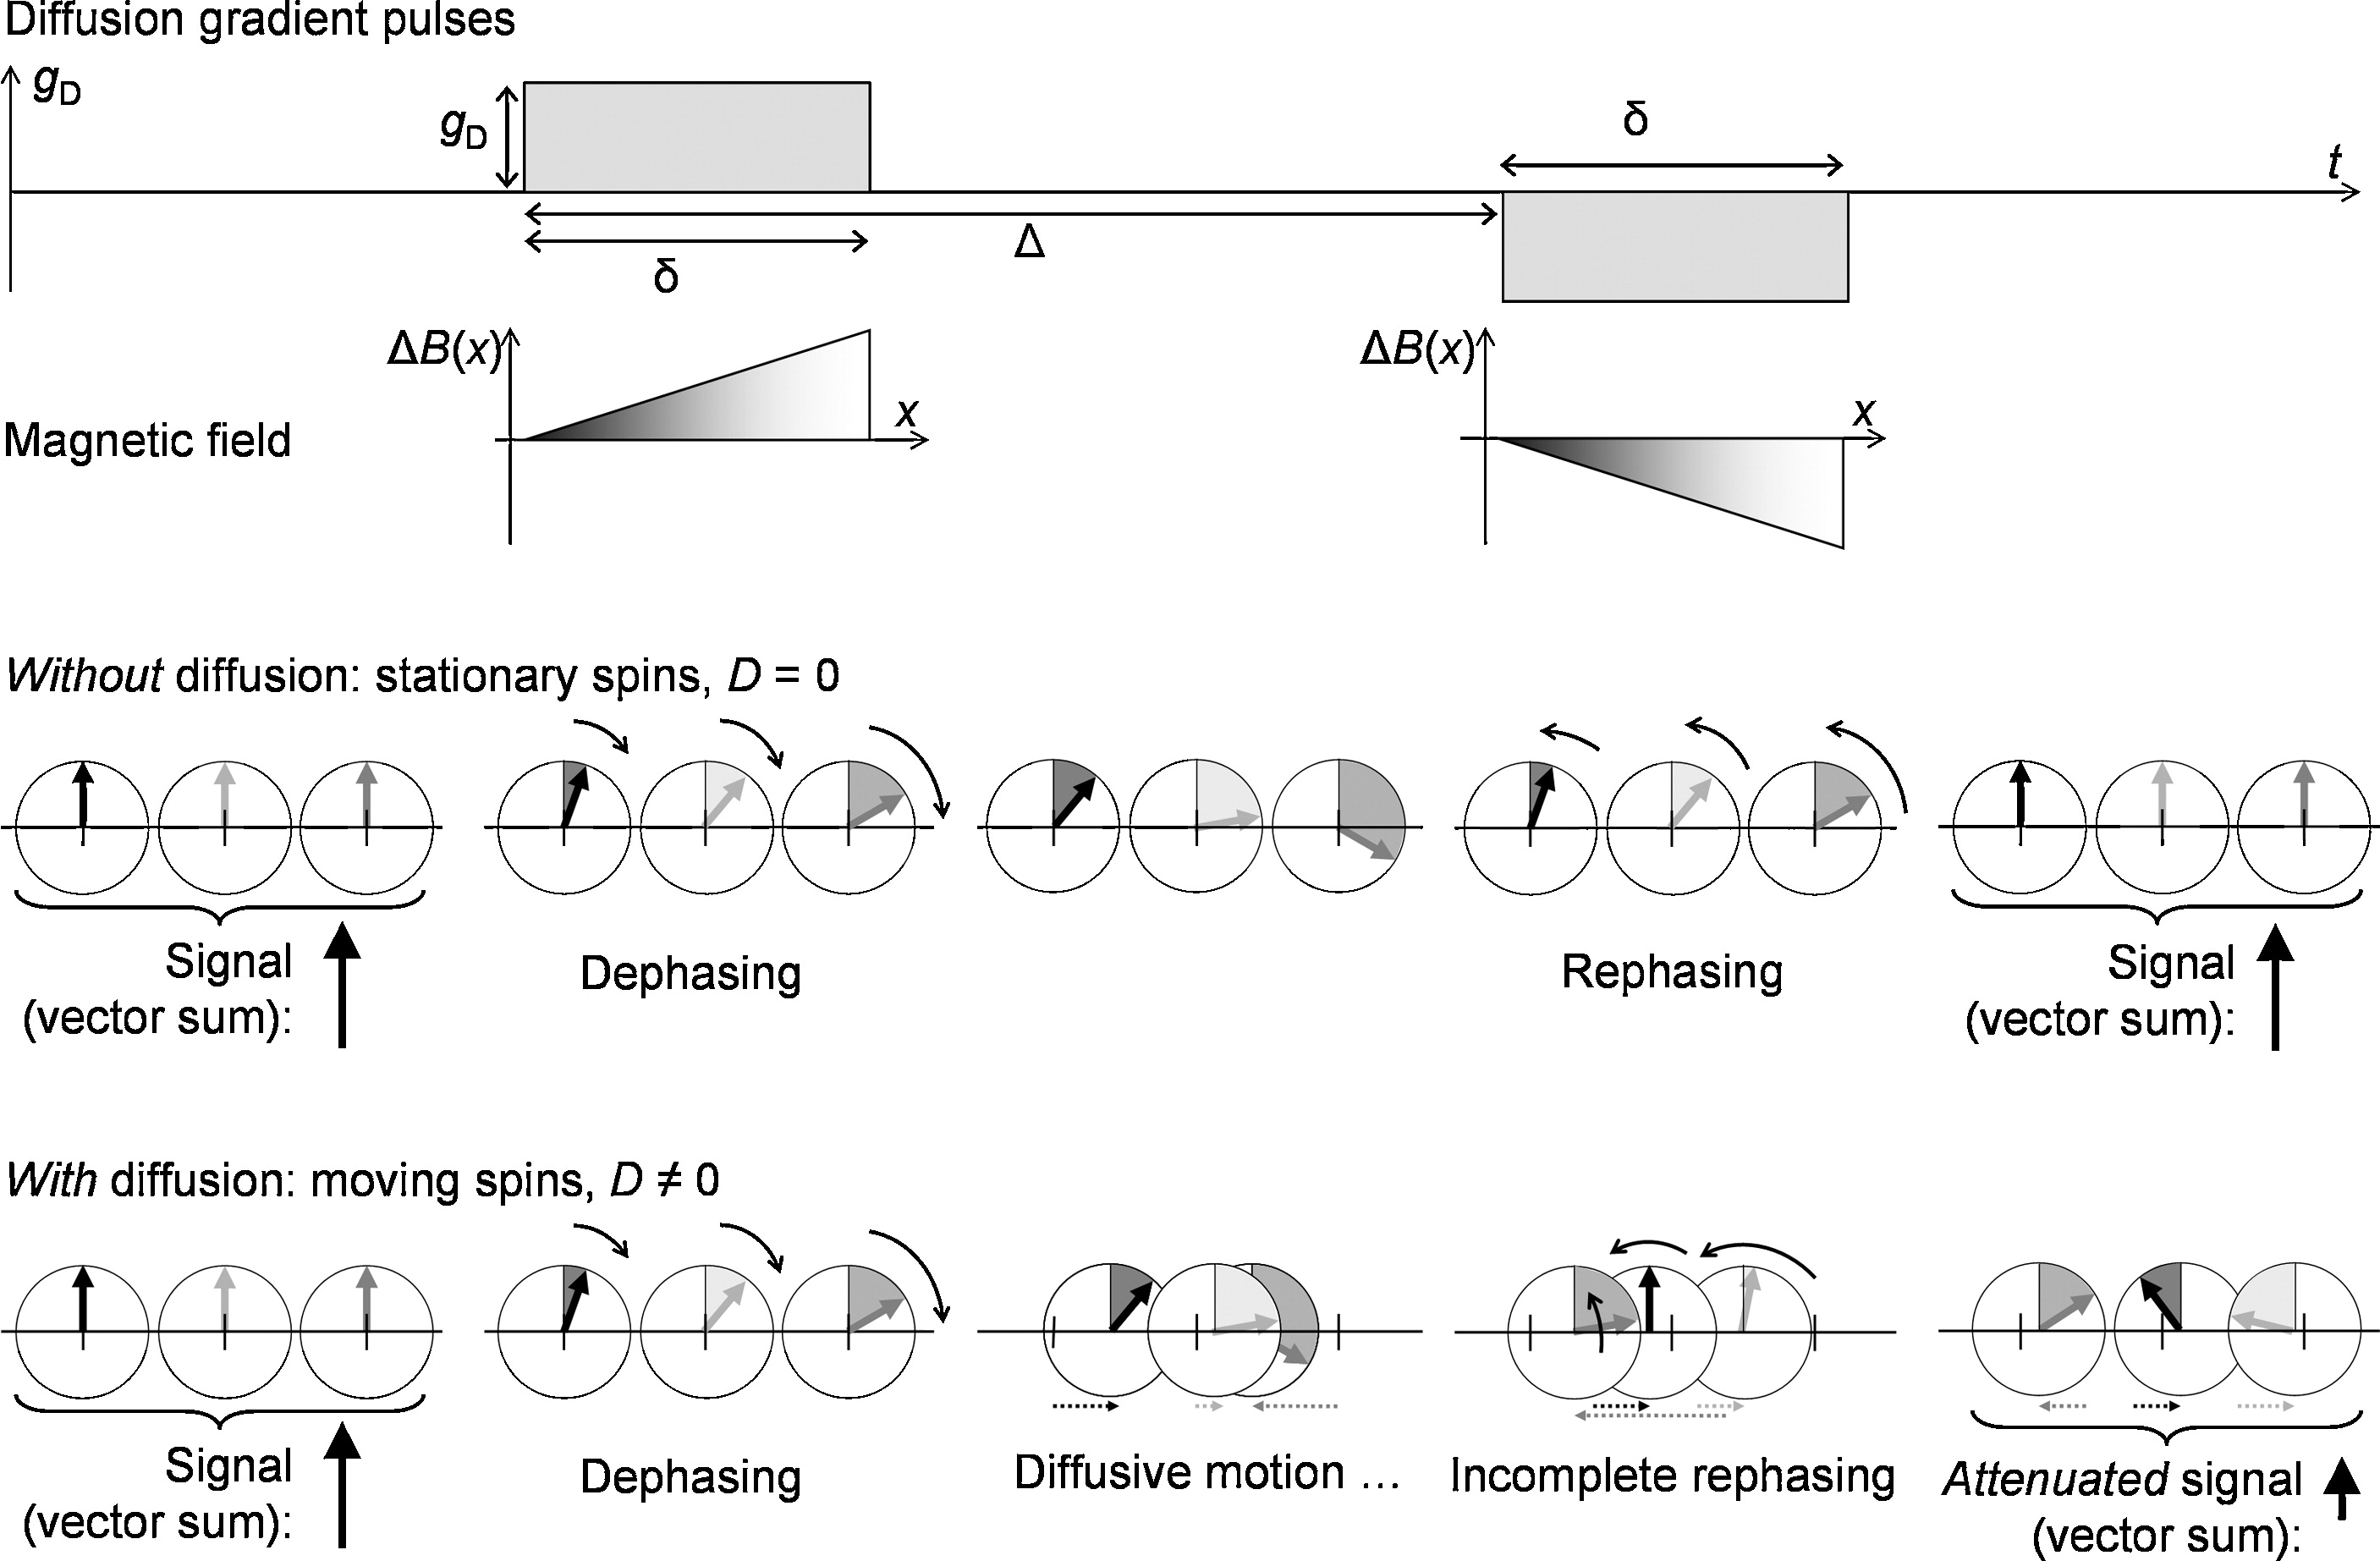
\includegraphics[width=\textwidth]{images/diffusionmri.jpg}
    \caption{Image from \cite{technical_aspects_dmri} elucidating the technical aspects of Diffusion Weighted MRI. The RF pulse causes a phase change of the net magnetization. Introducing the diffusion gradient adds spatial dependence of phase shift on the individual magnetic moments. The molecules that have restricted diffusion do not experience the effect of the diffusion gradient. Any phase change from the first gradient is reversed by the second. They tend to relax to their equilibrium state. However, the molecules that undergo free diffusion experience the effects of the diffusion gradients introduced by the second RF pulse (180 degrees) and hence will undergo a total phase shift dependent on the spatial location. This shift is manifested in terms of signal attenuation. The degree of signal attenuation depends on multiple factors as shown in \cref{eq:Stetjskal}.}
    \label{fig:diffmri}
\end{figure}
\label{sec:DWI}
In \gls{DWI} the intensity of each voxel represents the rate of water diffusion in a cubic region. Diffusion weighting is applied in order to generate contrasts based on the assumption that diffusion varies with pathology i.e. differences in diffusion can also highlight differences in structure and function \citep{Taylor_1985}. 

One of the most popular ways to give images diffusion weighting is by using \gls{SE} T2 weighted sequences with two symmetric gradients on each side of the 180 degree refocusing pulse. This is based on the \gls{PGSE} technique developed by \cite{stejskal1965spin}. \Gls{PGSE} improved sensitivity to diffusion in comparison to the steady state gradients used previously. \cite{stejskal1965spin} solved the Bloch-Torrey partial differential equations for a symmetric pair of pulsed gradients \citep{bloch1946nuclear} and obtained the well-known Stejskal-Tanner formula:
\begin{equation}
\label{eq:Stetjskal}
S = S_0 \exp^{-bD}
\end{equation}
Here $S_0$ represents the original signal strength, $S$ is the signal strength in a pulse sequence with the presence of diffusion gradients ($g_D$) and $D$ represents the diffusion coefficient. The attenuation of the \gls{dMRI} signal by the diffusion gradients is represented in \cref{fig:diffmri}. The application of the diffusion gradient results in a spatial encoding as the Larmour frequency becomes dependent on the net magnetic field (\cref{eq:larmour_grad}). In \cref{fig:diffmri}, it is evident that the Diffusion gradients are magnetic field gradients along the $x$ direction. 

Here $\Delta B_(x) = g_D x$, which makes the Larmour frequency spatially dependent $\Delta \omega = \gamma \Delta B_(x)$ or $\Delta \omega = \gamma g_D x$. There is a phase shift introduced after the gradient pulse of time duration $\delta$. The the phase shift is also dependent on the $x$ position due to the spatial dependence represented as $\Delta w(x)$ , the phase shift is $\Delta \phi (x) = \Delta w \delta = \gamma g_D x \delta$. This spatial dependence of the phase shift makes spins at different positions along the gradient axis ``dephased'' after the application of the gradient pulse. When the negative gradient is applied, the process of rephasing occurs. The dephasing and rephasing mechanisms result in the diffusion weighting of the image. Without any diffusion stationary spins would align along their equilibrium position (cancelling effect of the two opposing diffusion gradients) while with diffusion weighting there is a signal attenuation explained by \cref{eq:Stetjskal}. 

The b value of the diffusion weighted signal mentioned in \cref{eq:Stetjskal} is defined in the units of $s/mm^2$ as
\begin{equation}
    b = (\gamma g_D \delta)^2 (\Delta - \frac{\delta}{3})
\end{equation}
In order to obtain the numerical value of b, long and strong gradients are required. The diffusion gradients $g_D$, time of pulse $\delta$ and time interval $\Delta$ are often adjusted to adjust the b values. Higher b values leads to lower signal in the areas of high diffusion and increases the contrast between tissues that have different diffusion coefficients. The b values often need to be adjusted to obtain an optimal \gls{SNR}.


\subsubsection{Diffusion Tensor Model}
\label{subsec:DTI}
\gls{DTI} is a new type of imaging technique that relies on a tensor model to measure the diffusion on per voxel basis. Instead of attributing diffusion inside a voxel by to a single quantity, it uses a tensor formalism to measure diffusion along different directions within a voxel. The tensor model gives a rotationally invariant description of water diffusion. With this framework \gls{DTI} is hence able to trace complex fiber tracts in the brain \citep{jones2010diffusion}.

\gls{DTI} is a novel technology, an \textit{in-vivo} application of DWI and is the gold standard for imaging neural fiber tracts. It has become an important brain imaging modality since various neurological disorders such as cerebral ischemia and Parkinson’s disease can be attributed to white matter defects. Further, white matter constitutes about 50\% of the brain (by volume) which makes it important to understand both its structure and tissue composition. Analyzing structural brain connectivity using \gls{DTI} does not only help to understand the patho-physiological effect of brain disorders but also the structure of its functional networks.

In this type of imaging, each voxel is associated with a $3 \times 3$ diffusion tensor representing the diffusion of water molecules using a Gaussian model. It is symmetric and contains six unique variables that characterize diffusion (as anisotropic or isotropic). This tensor has 3 eigenvalues and 3 corresponding eigenvectors which represent the directions of diffusion along the voxel. The voxels are usually $1 mm^3$ in size and often constitute components of more than one cell within them. The diffusion tensor can be written as:
\begin{equation}
D =
\begin{pmatrix}
D_{xx} & D_{xy} & D_{xz} \\
D_{yx} & D_{yy} & D_{yz} \\
D_{zx} & D_{zy} & D_{zz}
\end{pmatrix}  
\label{mat:difftensor}
\end{equation}

where $D_{xy} = D_{yx}$, $D_{zy}=D_{yz}$ and $D_{xz}=D_{zx}$
In this case \autoref{eq:Stetjskal} can be written as 
\begin{equation}
\frac{S}{S_0} = \exp^{-bg^T Dg}
\end{equation}where $g^T$ is a $3 \times 1$ unit vector representing the gradient direction.
The cellular environment is heterogeneous, so water molecules in certain parts undergo free diffusion while in others they undergo restricted diffusion. Due to this restricted diffusion the measured diffusion coefficient (of the water molecules) is different from the regular diffusion coefficient of water, it is termed as the \gls{ADC}. Diffusion in complex environments cannot be explained by using diffusion gradients in one direction only. \Cref{fig:diffmri} shows that only the component along the gradient direction is detected. Therefore, it is required to apply diffusion gradients in three directions to get an estimate of anisotropy of water molecules. Diffusion anisotropy in a voxel means the deviation of the voxel diffusion from isotropic diffusion. High diffusion anisotropy means that there is a preferred direction for the water molecules within that voxels to diffuse \citep{clark2011mean}.

\gls{DTI} images are usually represented by either encoding the tensor information using a scalar (for intensity values in a black and white image) or 4 numbers (\gls{RGB} and brightness). Visually, the tensors can also be viewed as glyphs and very famously by tracing white matter tracts through a process known as tractography. The quantities such as \gls{MD} and \gls{ADC} are used to characterize diffusion magnitude. Other scalars such as \gls{FA} are used to characterize diffusion anisotropy. 

\gls{MD} is calculated as the trace of the diffusion tensor (Eq. \ref{mat:difftensor}). The \gls{FA} determines an average ratio of diffusion distortion from the applied gradient directions. In order to calculate the FA, the diffusion tensor is converted to a diagonal matrix (which has eigenvalues D1, D2, D3 the diffusion coefficients along x, y and z directions). \\
\begin{equation*}
D =
 \begin{pmatrix}
D1 & 0 & 0 \\
0 & D2 & 0 \\
0 & 0 & D3
\end{pmatrix}   
\end{equation*}

\begin{equation}
\label{eq:meanFA}
FA = \sqrt{\frac{3}{2}} \frac{\sqrt{(D1 -D_{mean})^2+(D2 -D_{mean})^2 + (D3 -D_{mean})^2
}}{\sqrt{D1^2 + D2^2 + D3^2}}
\end{equation}

Where D1, D2, and D3 are the corresponding eigenvalues and v1,v2,v3 are the eigenvectors.
\gls{DTI} is a popular method to study the orientation and organisation of white matter. However, it fails in regions containing populations of fiber orientations that have different fiber orientations. It assumes that all white matter bundles in the brain have similar diffusion characteristics and attributes diffusion anisotropy to partial volume effects \citep{tournier2004direct}. Secondly, the diffusion tensor only possess a single major eigenvalue for modelling the diffusion in one voxel and cannot be used for mixed fiber populations.
\subsubsection{Higher Order Models}
\label{sec:highermodels}

In order to solve the multiple fiber orientation problem of \gls{DTI} mentioned in \autoref{subsec:DTI}, a number of approaches have been proposed to estimate the composition of fiber orientations inside a voxel. These models extract higher order structural information of tissues. They can help deal with problems such as kissing and crossing fibers. 

\gls{HARDI} techniques fall into the class of higher order models since they enable the detection of multi-modal diffusion signals. They include methods that incorporate the acquisition of diffusion data in more than 6 diffusion gradient directions. Q-ball imaging is one such technique but has its own limitations \citep{TOURNIER20041176}. These methods rely on the concept of a \gls{fODF}. An \gls{fODF} is a symmetric probability distribution function describing the distribution of fiber orientations
\begin{align}
  F(\Theta, \phi) = \sum_{k=1}^{K} w_k \delta_{\theta_k, \phi_k}(\Theta, \phi) &
 & \Theta \in [0, \pi], \phi \in [0,2\pi]
\end{align}
where $w_k$ represents the volume fraction of each fiber passing through the voxel. $\Theta_k$ and $\phi_k$ represent the polar and azimuthal angles in spherical coordinates respectively.

To overcome the limitations of methods such as q-ball imaging, \cite{tournier2004direct} propose modelling the \gls{DWI} signal as the spherical convolution (i.e. convolution in spherical coordinates) of the response function and the \gls{fODF}. A response function is mathematically an axially symmetric kernel which describes the \gls{DWI} signal resulting from water diffusion along each fiber bundle aligned with the z-axis in a voxel. A different response function is estimated for different fiber populations such as \gls{WM}, \gls{GM} as \gls{CSF}.

\gls{SD} \citep{dell2019modelling} is a method in which the \gls{fODF} can be extracted by deconvolving the response function from the \gls{DWI} signal. \Gls{CSD} has also gained recent attention as a method to extract \gls{WM} fiber orientation distributions as it imposes constraints to remove negative values in the reconstructed \gls{fODF}. This increases the clinical feasibility and plausibility of the \gls{WM} tractography \citep{JEURISSEN2014411}.
%insert image

\subsubsection{Tractography}
\label{subsub:tractography}
\begin{figure}
    \centering
    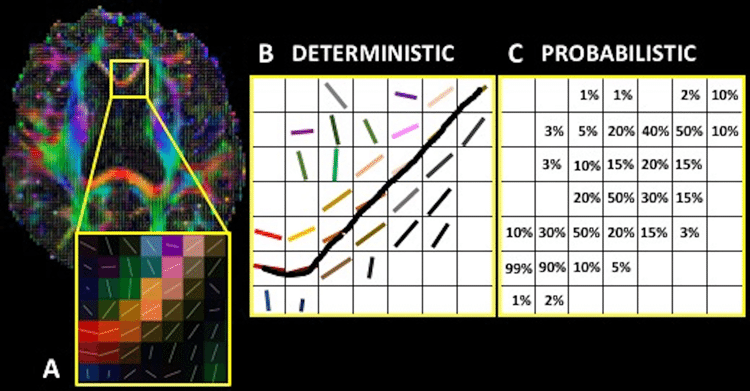
\includegraphics[width=0.7\textwidth]{images/A-Degree-of-anisotropy-B-Deterministic-fiber-tracking-the-fiber-path-across-voxels-is.png}
    \caption{Image from \cite{muller2018clinically} depicting different types of fiber tracking techniques. Red, green and blue regions indicate tracts running along the x, y and z axis respectively. (a) Depicts deterministic tracking where the largest eigenvector determines the direction of progression along adjacent voxels. (b) Probabilistic tractography is depicted. A probability distribution function represents multiple possible diffusion directions.}
    \label{fig:tracking}
\end{figure}
Fiber tractography is a technique used to graphically construct  3D representations of white matter pathways in the human brain. The technique uses the information about local fiber directions to trace streamlines that represent white matter tracts in the brain. It has become an important part of white matter disorder studies and has gained popularity because of its non-invasive nature. These advantages make it suitable for surgical targeting and planning \citep{romano2009pre}.

Tractography methods often use \gls{DTI} in order to delineate the streamlines along the white matter tracts. This is done by tracing the direction of diffusion from one voxel to the next. Fiber tracking relies on the assumption that the direction of maximum diffusion(in the diffusion tensor) aligns with the direction of the white matter fiber within the voxel. Tractography can be divided into two classes: deterministic and probabilistic tractography.

In deterministic tractography, the algorithm usually follows the direction of maximum diffusion from along the voxels by starting from a “seed” region. If the angle between two subsequent directions of maximum diffusion is less than predefined threshold, the algorithm proceeds tracking along the maximum diffusion direction of the second voxel and terminates when the condition is not met \citep{descoteaux2008deterministic}. The deterministic tractography does not take into account any random or systematic errors that arise during signal acquisition, recording and transmission.

Probabilistic tractography relies on the estimation of a \gls{PDF} such as an \gls{fODF} for the distribution of fiber orientations in each voxel. This helps to account for the possibility of crossing fibers and kissing fibers. The \gls{PDF}s and uncertainty are then used to build a path probability map corresponding to a seed point. Let's say N streamlines are propagated randomly from a seed point using an orientation along the distribution functions. For any to voxels A and B 
\begin{align*}
P_{AB}= \frac{M}{N} & \textrm{ , probability that a curve starting at voxel A passes through voxel B} \\
M = & \textrm{ number of streamlines that go through B and A} \\
N = &\textrm{ total number of streamlines generated from A}
\end{align*}
Using this probability map the most probable fiber orientation can be determined. From the multiple fiber orientations existing in a voxel the one most compatible with the incoming trajectory is chosen \citep{behrens2003non}.
\section[Brain Graph Representation]{Analyzing the Brain as a Graph}
\label{sec:braingraph}
The human brain is one of the most intricate biological systems. It has been well established this complex system can be modeled as a network composed of various dynamically interacting elements. The networks perspective has gained tractable attention in neuroscience and given rise to an ever expanding field of network neuroscience. Brain organization can vary at scale i.e. from molecular interactions to cognition. With different interactions and emergent properties at each level of organization, graph theory has become an indispensable tool in this field \citep{sporns2018graph}. 

Brain networks can be effectively represented as graphs for computational analysis. In the graphical representations, each node could represent an entire brain region or an individual neuron. Edges can be binary or weighted, directed or undirected. The architecture and properties of the graph depend on the scale and the nature of interactions being considered \citep{rubinov2010complex}. 

The widespread application of graph theory in neuroscience has given rise to the field of \textit{connectomics} \citep{sporns2005human} aimed at the analysis of the structural and functional brain connectivity. The structural networks usually represent the anatomy of the brain and are temporally stable (ignoring the effects of plasticity and development). On the other hand, the functional networks are temporally variable and dense. Structural networks are preferred when trying to study the physical nature of the brain and it's anatomy when trying to predict neurological disorders and searching the biochemical basis of cognition.

\iffalse
A graph can be defined as mathematical representation of pairwise relationships between objects. A graph is said to consist of two basic elements i.e. nodes (representing the objects themselves) and edges (representing the relationships between the nodes). 
\fi

\subsection{Connectomics}
\label{sec:connectomics}
\textit{Connectomics} is termed as the study of the brain's functional and structural networks. A connectome (in-vivo, retraced from imaging) is a dense network of brain connections, with a numerical value assigned to each network \citep{bassett2017network}. The connectome of a brain can be seen as a circuit diagram with the neural connections analogous to wires and the cell bodies to electrical components.

Recently connectomics has become the focus of major neuroscience studies. Research in this field has expanded rapidly due to the increasing interest in understanding the brain as a dynamic system, and the belief that its connections give rise to its capabilities and functionality \citep{network_neuroscience_editorial}.

The first complete structural connectome to be mapped at the synaptic level was published in 1986 and belongs to the species C. elegans. It was reconstructed using electron micrographs of the serial section. It is a network that possesses three hundred neurons and roughly seven thousand connections. After 1986, it still took decades to claim the biological plausibility of all the connections in the reconstructed connectome \citep{elegans}. This trend lead to the conclusion that the connectome of the human brain cannot be mapped using the manual labor-intensive methodology employed by \cite{white1986structure}. The human brain contains roughly the same number of neurons as the stars in the Milkyway galaxy and about $10^{15}$ inter-neuronal connections called synapses \citep{fornito2015connectomics}. Mapping the human brain manually seems implausible in terms of time considerations. This calls for the need to computationally determine brain connectivity from brain scans.

\gls{dMRI} is used for the construction of the structural connectome while \gls{fMRI} is the preferred modality for functional connectome construction. The \gls{HCP} was launched in 2007 as the first large scale collaborative effort to create detailed maps of the brain (in-vivo) and to help better understand the fundamentals of human connectional anatomy.

\subsection{Structural Brain Connectivity}
Structural brain connectivity refers to the arrangement of anatomical connections in the brain. A model of the brain's structural connectivity can be derived from whole brain tractography. In organisms with complex nervous systems such as that of humans, the structural brain connectivity can be visualized at different scales. It can be either at the level of synaptic connections (microscale), at the level of neuronal populations (meso-scale) or at macro scale in which fiber tracts run between different brain regions. At all these scales, the connectivity patterns of individuals from the same species exhibit different characteristics such as organization, topology and spatial extent \citep{Sporns:2007}.

In neuroimaging studies the connectivity is usually analyzed at the macroscopic scale, i.e. fibers that run in between different brain regions are traced. From  \autoref{subsub:tractography} it can be inferred that the streamlines traced using the tractography algorithms represent the structural connections between different \gls{ROI}s of the brain that are represented as brain nodes. The ROI-to-ROI connections are usually represented using bio-physical parameters such as mean \gls{FA}, number of streamlines between the two nodes and the length of the streamlines connecting the two nodes.
\section{Feature Selection Techniques}
\vspace{-0.5em}
\label{sec:feature_selection}
Neuroimaging data often suffers from the \textit{curse of dimensionality}. The sample size is often much smaller than the total number of features. Classifiers might be influenced by the increase in noise as the number of features increases. Dimensionality reduction and feature selection are often the techniques used for a meaningful reduction in features. However, most dimensionality reduction methods such as \gls{PCA} rely on transformations of the original data and do not provide interpretable features. Due to this reason, it is important to consider feature selection methods where inference about which features the classifier learns can be made \citep{shi2018feature}.

Feature selection methods can be grouped into three types: filter methods, wrapper methods and embedded methods. Filter methods are based on selecting features before running the classifier. Wrapper methods can be seen as a selection method which select features \textit{on the fly} i.e. features are added or removed iteratively on the basis of classification performance. Embedded methods are those in which feature selection is embedded in the classifier. All three types of are being increasingly used in neuroimaging studies, however filter methods remain advantageous due to interpretability considerations \citep{tohka2016comparison}. The remainder of this section will focus on filter methods due to their relevance in the methodology of this thesis.

Filters form one of the simplest methods for feature selection. They usually serve as a preprocessing step for the classification and are model independent. However, there is a caveat in using such techniques for classification studies. The caveat is that each raw feature is considered independently and the cumulative effect of separate features is not taken into consideration for selection. One of the common techniques used to determine feature importances is the use of coefficients such as the f-scores, t-test and Pearson correlation coefficients which are widely used in neuroimaging applications \citep{mwangi2014review}.

Assume a two class classification task. In such a task the subjects can be divided into two groups. When the sample size is equal, a two independent samples t-test is a natural choice to compare the group differences. In such a case the null hypothesis remains that the means of the feature for the two groups is the same. Based on \cite{inza2004filter}, the t-statistic is calculated as:
\begin{align}
        \label{eqn:tstat ind}
       t &= \frac{|\overline{x_1} - \overline{x_2}|}{\sigma_{p}*\sqrt{\frac{2}{n}}} \\
       \sigma_p &= {\sqrt{(\frac{\sigma_{1}^2 }{n_{1}}+ \frac{\sigma_{2}^2}{n_{2}})}}
\end{align}
When the sample size of two groups are unequal. A Welsch's t-test can be carried out in cases where it can be assumed that the two groups have similar variances. The t-statistic is then given as:  
\begin{align}
    \label{eqn:tstat welsch}
    t &= \frac{|\overline{x_1} - \overline{x_2}|}{(\sqrt{\frac{1}{n_{1}}+\frac{1}{n_{2}})}*\sigma_p} \\
    \sigma_p &= \sqrt{\frac{(n_{1} -1) * \sigma_1^2 + (n_{2}-1) * \sigma_2^2}{n_{1} + n_{2} -2}}  
\end{align}
For both the t-statistics, $\sigma_{1}$ represents standard deviation for the feature values of the first group, $\sigma_{2}$ is the value for the second group, $\sigma_p$ is the pooled standard deviation, and $n_{1}$, $n_{2}$ represent the number of samples for class 1 and 2 respectively. The features can be ranked on the basis of the p value of the t-test to obtain its statistical significance. Typically, values of $p<0.05$ are considered statistically significant \citep{colquhoun2017reproducibility} and only then can the null hypothesis can be rejected with confidence. Furthermore, using a t-statistic the population parameters can be estimated for a particular feature. 

The t-tests have a number of limitations. One of the most prominent limitations is that can only be implemented for two group differences. F-scores can overcome this limitation and can be used to rank features for two or more groups. Mathematically, the f-score can be defined as: 
\begin{equation}
\label{eq:fscores}
    F = \frac{\sum_{j=1}^{K}(\overline{x_{j}} - \overline{x})^2 }
    {\frac{\sum_{j=1}^{K}\sum_{i=1}^{n1}(x_{j,i} - \overline{x_{1}})^2}{n_{j} -1}}
\end{equation}
where $\overline{x}$ represents the average value of the feature for all groups, $\overline{x_{j}}$ the feature average for for the $k_th$ class.

The f-scores measures the ratio of between group variances to within group variances and the p-value of the t-test measures if the differences between the means of two groups are statistically significant. These two scoring techniques can be used to verify if the ranking generated by one corresponds to that generated by the other.

Based on a similar concept, the Pearson correlation coefficient can be used to filter features if the target variables are continuous. The Pearson correlation coefficient is defined as: 
\begin{equation}
    \rho = \frac{\sum_{i=1}^{N} (x_{i} - \overline{x}) (y_{i} - \overline{y})}
    {\sqrt{\sum_{i=1}^{N} (x_{i}-\overline{x})^2 \sum_{i=1}^{N} (y_{i}-\overline{y}^2)}}
\end{equation}
where $y$ represents the target variable and $N$ represents the total number of data points. This takes the linear relationship between the feature values and the target variables into account.
\iffalse
Numerical thresholds can also be applied for feature ranking if such a method-ology is suited to the nature of the problem
\fi

\section[MWCS]{Maximum Weight Connected Subgraph}
\label{sec:MEWS}
Finding discriminative subgraphs representing interaction networks is an important problem in bioinformatics. One effective way of find such subgraphs is by solving the \gls{MWCS} problem. The major aim of the \gls{MWCS} problem is to find a connected subgraph with the maximal sum of node weights \citep{DBLP:journals/corr/LobodaAS16}.

\gls{MWCS} problem falls into the class of NP-hard problems. Given a connected and undirected graph $G=(V,E)$, the \gls{MWCS} can be defined as that subgraph $G=(\tilde{V}, \tilde{E})$ which satisfies the equation:
\begin{equation}
    \Omega (\tilde{G}) = \sum_{v \in \tilde{V}} w_v \longrightarrow max
\end{equation}
where $w_v$ is the weight of a node $v$.

There are many variants of this problem which are used for specific applications. For example, a cardinality-constrained \gls{MWCS} is used in systems biology to detect core components in gene networks \citep{yamamoto2009better}. Analogously, a directed \gls{MWCS} has been used to find the most deregulated networks in biological pathways. In both these cases the core networks are determined to be the ones which have maximum sum of the node weights \citep{backes2012integer}.

The above stated implementations are not well suited for analysis of brain networks since connection strengths are of high importance in such a task. There has to be an account of similarity between nodes in order to get interpretable subgraphs. In such a case a generalized MWCS (GMWCS) based on the MWCS but with consideration of edge weights is suitable. The mathematical explanation for the generalized \gls{MWCS} (GMWCS) will be presented in the remainder of this section.

\iffalse 
This method is widely used in biological network enrichment analysis \citep{DBLP:journals/corr/LobodaAS16}. One important application of this technique is to detect deferentially regulated pathways based on environmental or phenotypical changes \citep{althaus2014algorithms}.
Another application arises in the area of system biology [8,22, 1]. Yamamotoet al. [22] suggest the cardinality-constrained MWCS in order to detect core sourcecomponents in gene networks, which seem to be responsible for the difference be-tween normal cells and mutant cells. The input graphs are constructed from generegulation networks combined with gene expression data provided as node weights.Maximum weight connected subgraphs are considered to be good candidates forthese  core  source  components. A  directed  version  of  the  MWCS has  been  con-sidered in Backes et al. [1], where the most deregulated connected subnetwork inregulatory pathways with the highest sum of node scores (arising from expressiondata) is searched. In their model, they call a subgraph connected if all the nodes arereachable from one node, also called therootin the subgraph. The detected rootsare likely to be the molecularkey-playersof the observed deregulation
In dense networks such as the brain networks, a large number of interactions take place and it is difficult to keep a track of which interaction is important for a particular phenomenon. It consists in identifying the biologically relevant expression changes, the "big picture" of the experiment. We need to find subnetworks important for the phenomenon we want to study. It can be extended to analyse brain networks to determine brain pathways which are correlated to a particular behavioral measurement/ physiological or epigenetic character.
\fi

Consider an undirected, connected graph $G = (V,E)$ with weighted nodes and edges. The weighting can either be positive or negative. Let $V$ represent the set of its vertices, $E$ the set of its nodes, $w_e$ the weight of an edge $e$ and $w_v$ the weight of a node $v$. Mathematically, the \gls{GMWCS} can be described as that subgraph  $\Tilde{G} = (\Tilde{V}, \Tilde{E})$ which maximizes the following function:
\begin{equation}
\label{eq:sumfun}
    \Omega(\Tilde{G}) = \sum_{v \in \Tilde{V}} w_v + \sum_{e \in \Tilde{E}} w_e \longrightarrow max
\end{equation}

Extracting such a subgraph can be a useful feature selection technique in connectomics. The usage of this method as a feature selection technique can help overcome the limitations of filter methods in neuroimaging. Filter methods do not incorporate spatial patters and interactions of multiple features \citep{behrens2003non}. Furthermore, there is a requirement to find a suitable thresholds for statistics such as p-value and t-statistic for which no ground truth is available. An implementation that finds a subgraph satisfying \cref{eq:sumfun} eliminates the need to threshold and also takes the node interactions into account. Hence the \gls{GMWCS} can be used as a feature selection technique in connectomics.

According to the conceptual framework in \cite{DBLP:journals/corr/LobodaAS16}, the \gls{GMWCS} problem can be formulated using a \gls{MIP} formulation. By using a mixture of integral and binary variables, the maximal value of the objective function (Eq. \ref{eq:sumfun}) can be optimally found using a set of constraints.

The first step of formulating such a problem is to represent a candidate optimal subgraph. The membership of nodes and vertices in the subgraph is represented using binary variables:
\begin{align}
    \label{eq:y_v}
    y_v = 1  \iff v \in V  \textrm{ and } v \in \Tilde{V} \\
    \label{eq:w_e}
    w_e =1  \iff e \in E  \textrm{  and }  e \in \Tilde{E}
\end{align}
Conceptually, an edge should be present in the subgraph only if both the end vertices are also present in the subgraph. In \cref{eq:memberconstraint} this condition is represented as an inequality.
\begin{align}
    \label{eq:memberconstraint}
    w_e \leq y_v && \forall v \in V, e \in \delta_{v}
\end{align}
where $\delta_{v}$ represents the set of incoming edges on a node. Consider if $y_v = 0$, then $w_e$ has to be zero because an edge cannot be present without the node being present and if $y_v = 1$ then $w_e = 0$ or $w_e = 1$ because it is not necessary for an edge to be present if a node is present.

After the subgraph can be represented, it is important to establish the validity of a candidate subgraph. A valid \gls{GMWCS} needs to be connected and maximise the function \cref{eq:sumfun}. To establish the connectedness of the subgraph the concept of an arborescence needs to be introduced.

An arborescence is an acyclic directed graph in with a root node $v$, having exactly one path from $v$ to any other vertex $u$. The connectedness in a graph is defined as the existence of a simple path between any two nodes. For creating a valid connected subgraph, its traversal has to be a valid arborescence. The \gls{GMWCS} is constructed by finding a valid arborescence matching to its traversal.

The traversal of any graph can be found by considering $S = (V,A)$ derived from $G=(V,E)$  where each undirected edge $(v,u)$ is replaced by two directed arcs $(u,v)$ and $(v,u)$. To ensure the connectedness of the subgraph, a non-linear formulation is needed where:
\begin{itemize}
     \setlength\itemsep{0.5em}
    \item Binary variable $x_a = 1$ iff $a \in A$ belongs to the arborescence.
    \item Binary variable $r_v = 1$ iff $v \in V$ is the root of the arborescence,
    \item Continuous variable $d_v = n$ if the length of the simple path from the root to the vertex v is n. The $d_v$ value can be arbitrary if the vertex v does not belong to the optimal solution
\end{itemize}
As pointed above, a valid arborescence corresponds to the traversal of the connected subgraph. Hence, the arborescence needs satisfy the following constraints, according to \cite{haouari2013enhanced}:
\begin{align}
    \label{eq:rv}
    \sum_{v \in V} r_v = 1\\
    \label{eq:dv}
    1 \leq d_v \leq n && \forall v \in V \\
    \label{eq:uvrv}
    \sum_{(u,v) \in A} x_{uv} + r_v = y_v && \forall v \in V\\
    \label{eq:fronba}
    x_{uv} + x_{vu} \leq w_e && \forall e =(v,u) \in A\\
    \label{eq:dvrv}
    d_v r_v = r_v\\
    \label{eq:dudv}
    d_u x_{vu} = (d_v + 1) x_{vu} && \forall e=(v, u) \in A
\end{align}
 \Cref{eq:rv} ensures that there is only one root of the arborescence. \Cref{eq:dv} limits the path length from the root vertex to any other vertex in the arborescence if it is present in the subgraph. With \cref{eq:uvrv} it can be established if a vertex is a root then there are no incoming edges and that there is a maximum of one incoming edge on each node. The constraint in \cref{eq:fronba} says that either the forward arc or the backward arc can be a part of the valid arborescence and not both. The last two constraints in \crefrange{eq:dvrv}{eq:dudv} impose that the length of the path to the root is always 1 and the distance of the nodes correspond to the direction of the edges.
It can be seen that the \crefrange{eq:dvrv}{eq:dudv} are non-linear. Combining the above equations the linearization is as follows:
\begin{align}
    \label{eq:dvlin}
    d_v + n r_v \leq n && \forall v \in V\\
    \label{eq:nuvlin}
    n + d_u - d_v \geq (n+1) x_{vu} && \forall (v,u) \in A\\
    \label{eq:dvdulin}
    n + d_v - d_u \geq (n-1) x_{vu} && \forall (v,u) \in A
\end{align}
\Cref{eq:dvlin} combines \crefrange{eq:rv}{eq:dv}. \Crefrange{eq:nuvlin}{eq:dvdulin} can be justified using the fact that if a directed edge $(v,u)$ is present, then node $v$ is visited before node $u$ and $d_u - d_v = 1$. They hence represent the \cref{eq:dudv}.
Any arbitrary node is considered to be the root of such an arborescence. The valid arborescence is then used to construct the optimal \gls{MEWIS}.

\section{Classification}
An important task in connectomics is to analyze the differences between individuals using connectivity graphs. Machine learning algorithms have previously been used in combination with graphical representations in order to make predictions from neuroimaging data \citep{casanova2012combining}. This section describes three classifiers which are incorporated in the methodology of this work. 

\subsection{Support Vector Classifiers}
\begin{figure}[h]
    \centering
    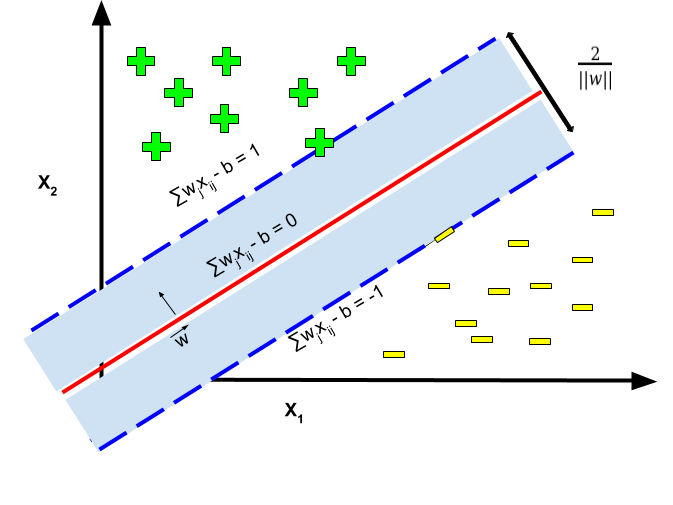
\includegraphics[width=0.65\textwidth]{images/SVM.png}
    \caption{Illustration of classification using \gls{SVM}s. The red line represents the decision boundary between the two classes. The algorithm maximizes the margin between the boundary for separate classes. The vectors lying on the hyperplanes depicted by the blue dashed lines are called as `support vectors' and are the closest vectors to the decision boundary. Based on the values obtained by solving the left hand side of the decision boundary for each data points, they are assigned to the corresponding classes.}
    \label{fig:svm}
\end{figure}
\gls{SVC} are classical machine learning algorithms based on \gls{SVM}s. They are important since they have attained significant accuracy with different types of tasks such as a handwritten digits recognition, face detection in images, and text categorization \citep{burges1998a}. In neuroimaging studies, SVCs are important for classification tasks since they are relatively robust to overfitting and more interpretable than Deep Learning classifiers.

In the simplest, binary case the mathematical formulation of the SVM is as follows. Consider each observation \textbf{$x_i$}, $i\in {1...n}$ to be a vector in the \textit{d-dimensional} feature space with a target label  $y_i\in {[-1,1]}$. The classifier needs to find a boundary that separates \textit{n} such points present in the presented data within a small margin of error. It does so by trying to find an optimally separating hyperplane that efficiently divides the input data according to the target labels. In \cref{fig:svm} the red line represents the optimally separating hyperplane that satisfies the equation
$ \sum w_i x_i - b = 0$
 It is maximally distant to the nearest point belonging to either class (also termed as the support vectors). The maximally separating hyperplane is found by satisfying the following constraints for each data point i. 
\begin{align}
    y_i(\sum_{j=1}^{d} w_{j} x_{ij}  + b)  - 1\geq 0 && \forall i \in {1...n}
\end{align}
Here, the weights represent the parameters the model learns in order to satisfy the above conditions by solving a Langrangian equation, the mathematics of which is beyond the scope of this text. 

In cases where the decision boundary is a non-linear function of the data the algorithm makes uses of what is commonly called as the `kernel trick'. In this method the pairwise dot products of the individual $x_i$ are replaced by a non-linear transformation or kernel function. This expression then allows the algorithm to fit the maximum margin hyperplane in the transformed space. The decision boundary is linear in the transformed space and can be projected back to find the non-linear decision boundary in the original $d$ dimensional feature space. 
\begin{figure}[h]
    \centering
    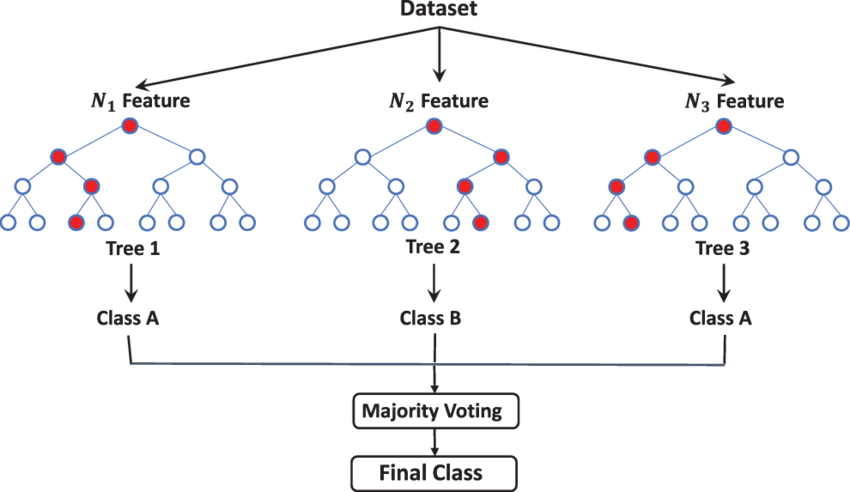
\includegraphics[width=0.75\textwidth]{images/Random_forest.png}
    \caption{Schematic explanation of Random Forest classifier from \cite{TAHMASEBI2020103619}. The different trees represent the decision trees constructed from the bootstrapped samples. Each tree is created on the basis of the most discriminatory features, $N_x$ for a particular bootstrapped sample. The final class of the samples in the dataset is decided on the basis of majority voting.}
    \label{fig:random_forests}
\end{figure}
\subsection{Random Forest Classifiers}

\gls{RF2} Classifiers are based on the idea of bagging or bootstrap aggregation of decision trees \citep{hastie2009elements}. A decision tree is a way of recursively splitting the target variables on the basis of the rules set on the features. The name `Random Forest' comes from the fact that the algorithm builds a `forest' by aggregating a large number of de-correlated trees and averages them for building a classification. 

The Random Forest is built in the following manner. A number of runs is specified. First, a bootstrap sample is drawn from training data. On this bootstrapped data, one tree is grown by recursively splitting the tree tree until the minimum node size $n_{min}$ is reached. The steps for the recursive decision tree construction are:
\begin{itemize}
    \item Select $k$ variables randomly from the $p$ total variables.
    \item Find the most predictive variable that has the most discriminatory split point.
    \item Split the node into daughter nodes.

\end{itemize}
This method is repeated to obtain a decision tree for each time a bootstrapped sample is obtained. The individual trees are the aggregated to make an ensemble on the basis of the ensemble vote of each tree. It is evident from the \cref{fig:random_forests}, the final classification of samples is based on the majority voting and hence a feature importance can be determined. The higher the position of a split in the random forest tree, the higher is its discriminatory power. Random forest classifiers are widely used in neuroimaging studies due to the interpretability of features which can be obtained using the feature ranking in terms of the feature importance. 

\subsection{Multilayer Perceptron}
A \gls{MLP} is an \gls{ANN} that is organized in the form of layers to mimic biological neural networks. The network consists of an input layer, an output layer as well as one or more hidden layers as shown in \cref{fig:mlp}.b. Each layer consists of one or more artificial neurons (also called as perceptrons) which are connected to neurons of the subsequent layers. 

\begin{figure}
    \centering
    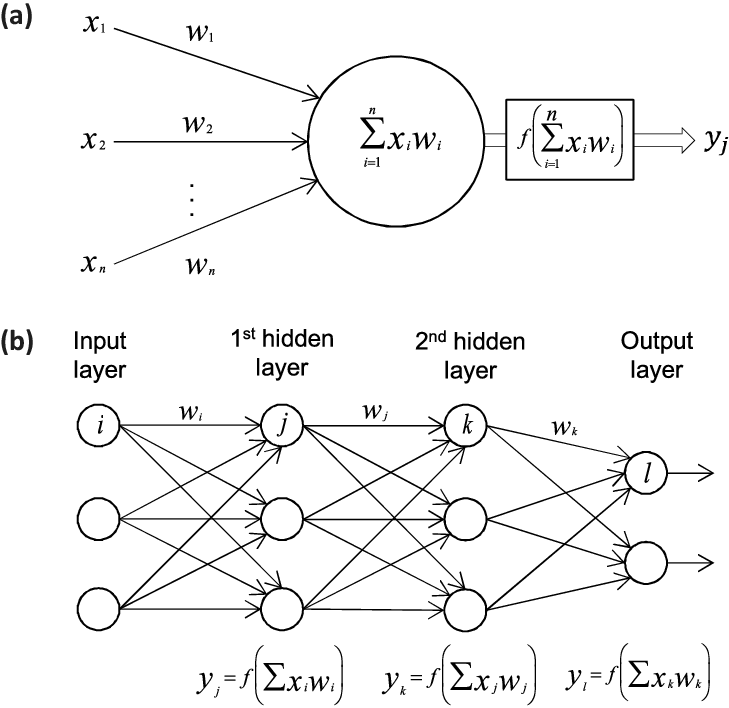
\includegraphics[width=0.5\textwidth]{images/tnn_ann.png}
    \caption{(a) Visualization of an artificial neuron from \cite{vieira2017using} depicting the output as a function of weighted sum of the inputs (Eq. \ref{eq:op_neuron}) (b). The artificial neural network consisting of the input layer, hidden layers and the output layer.}
    \label{fig:mlp}
\end{figure}
The connections between the layers are feed-forward and uni-directional. The input layer serves as a buffer layer with no transformation of the input while in the other layers the neurons implement non-linear transfer functions on the weighted connections from the previous layer as shown in \cref{fig:mlp}.a. The output $y$ from a neuron can be expressed as:
\begin{equation}
    \label{eq:op_neuron}
    y = g(\sum_{i=1}^{N} w_i x_i +b) 
\end{equation}
where $w_i$ represents the weighting of the inputs and b represents the bias for the neuron. Using the organizational structure, the neural network is able to learn complex transformations from the input data. In fact, it has been shown that an \gls{MLP} with just one hidden layer and a finite number of neurons is able to act as a universal function approximator \citep{universal_mlp}. Consider that we have an input vector in the N dimensional space and the output is needed in the M dimensional space. An \gls{MLP} (having non-linear transfer functional units) can implement any continuous mapping from the M dimensional space to the N dimensional space, with arbitrary accuracy. However, the number of neurons in the hidden layer required to achieve sufficient accuracy might be large which makes such a network difficult to train.

In order to achieve better accuracy and learn hierarchical representations, the network can be made `deep' by adding more layers. Additionally, increasing the depth of the network helps overcome the problem of overfitting in shallow neural network without the need to train on a large number of samples \citep{bengiodl}. Deep Learning is employed in neuroimaging studies in use-cases where there is a requirement to eliminate the need for manual feature selection.
\iffalse
What differentiates them from other classifiers, however, is the automatic feature learning from data which largely contributes to improvements in accuracy. This represents an important advantage and removes a level of subjectivity (e.g., the researcher typically has to decide which features should be tried) from existing approaches. With deep learning this subjective step is avoided.

Another distinguishing feature of deep learning is the depth of the models. Based on already acceptable feature learning results obtained by shallow models—currently dominating neuroimaging field—it is not immediately clear what benefits would depth have. Considering the state of multimodal learning, where models are either assumed to be the same for analyzed modalities (Moosmann et al., 2008) or cross-modal relations are sought at the (shallow) level of mixture coefficients (Liu and Calhoun, 2007), deeper models better fit the intuitive notion of cross-modality relations, as, for example, relations between genetics and phenotypes should be indirect, happening at a deeper conceptual level \citep{deeplearningneuroimg}.
\fi

\end{document}
